\begin{figure}
    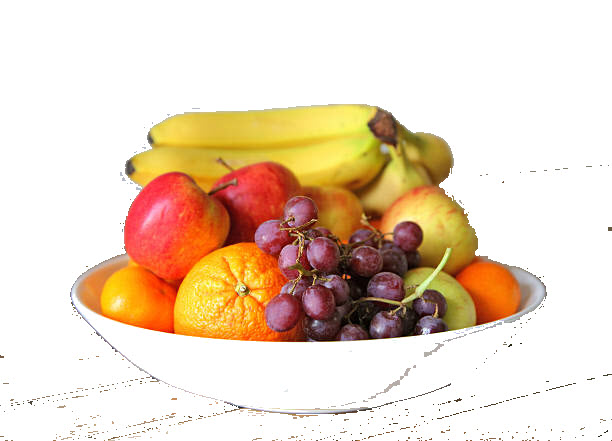
\includegraphics{fruitFillBg}
    \caption{Bowl of fruit with background removed}
    \label{fig:filledFruit}
\end{figure}

\begin{table}[]
    \centering
    \caption{Comparison of fruit image sliding window results with and without
    bakground}
    \label{comparisionFruitTable}
    \begin{tabular}{lllllll}
        Food type & Grid & Row & Column & Filled Grid & Filled Row & Filled
        Column \\
        Apple     & 5    & 1   & 3      & 10          & 0          & 4
        \\
        Banana    & 1    & 0   & 1      & 0           & 0          & 0
        \\
        Grape     & 4    & 0   & 0      & 1           & 0          & 1
        \\
        Orange    & 5    & 0   & 0      & 3           & 0          & 0
        \\
        Other     & 0    & 3   & 1      & 1           & 4          & 0            
    \end{tabular}
\end{table}

\subsection*{Overview}
As we can see in Experiment 9, using sliding windows to classify many sections
of an image, there were some cases where some unexpected predictions were made.
Due to this, the decision was made to analyse the effect the background of the
image has on its classification. The sliding window code was then ran on a new
image. This new image was the same fruit bowl as used previously but the
background was filled in as white as per Figure \ref{fig:filledFruit}.

\subsection*{Results}
\subsubsection*{Grid}
For grid based sliding window approach, the results turned out to be less
sucessful than with the background. In this experiment, fourteen out of fifteen
of top-1 classification were of an expected food type rather than fifteen out of
fifteen with the background present. We expected the food types of apple,
orange, grape and banana to appear in this image but while a banana was detected
to a top-5 accuracy on a few occasions it was never predicted to a top-1
accuracy. The contrast between the image results can be seen in Table
\ref{comparisionFruitTable}.

\subsubsection*{Row}
The row based sliding window again had worse result than its counterpart, with
zero out of four correct classifications as opposed to one. In this case, an
orange appeared at top-5 accuracy once. The most common prediction was ice-cream
which appeared at top-1 accuracy in three out of four instancs.

\subsubsection*{Column}
In contrast to our previous two methods of sliding window, this method
outperformed its counterpart with correct predictions of all five windows while
before we only had four out of five. In this experiment, a aple was predicted
four times and a grape once, with all correct fruits appearing to top-5
accuracy.

\subsection*{Empirical Analysis}
It is quite interesting that removing the background to the image reduced our
accuracy overall. Many white foods were classified instead which makes sense due
the impact of colour expected.
